\chapter{Building a Hidden Markov Model for Isolated Signs}
\ifpdf
    \graphicspath{{Chapter2/Chapter2Figs/PNG/}{Chapter2/Chapter2Figs/PDF/}{Chapter2/Chapter2Figs/}}
\else
    \graphicspath{{Chapter2/Chapter2Figs/EPS/}{Chapter2/Chapter2Figs/}}
\fi
% ------------------------------------------------------------------------

\section{Scaling}
In the previous section we introduced methods for solving the evaluation and re-estimation problems for hidden markov models. These methods, whilst mathematically sound, introduce certain problems during implementation. In particular these solutions involve the products of a large number of probabilities, especially for long observation sequence. As a consequence when implemented these methods can cause errors due to underflow. To solve this problem we instead scale the intermediate $\alpha$, $\beta$ and $\gamma$ variables to prevent underflow in the intermediate calculations and choose to compute the logarithm of the probability in the evaluation problem. To do this we normalize the $\alpha_t(i)$ by setting
\begin{align*}
\overline{\alpha}_0(i) = \alpha_0(i) \text{ for each $0\leq i<N$} 
\end{align*}
and inductively defining for each $0\leq t < T$
\begin{align*}
c_t &= \frac{1}{\sum_{i=0}^{N-1}\overline{\alpha}_t(i)}\\
\hat{\alpha}_t(i) &= c_t\overline{\alpha}_t(i)\text{ for each $i$}\\
\overline{\alpha}_{t+1}(i) &= \sum_{i=0}^{N-1}\hat{\alpha}_t(i)a_{ij}b_j(O_{t+1}) \text{ for each $i$}\\
\end{align*}
We then have
\begin{align*}
1 = \sum_{i=0}^{N}\hat{\alpha}_{T-1}(i) &= c_0c_1\dots c_{T-1}\sum_{i=0}^{N}\alpha_{T-i}(j)\\
&=c_0c_1\dots c_{T-1}\mathbb{P}(\mathbf{O}|\lambda)\\
\end{align*}
and hence we can compute the log-probability of an observation sequence $\mathbf{O}$ by
\begin{equation*}
\log(\mathbb{P}[\mathbf{O}|\lambda]) = -\sum_{t=0}^{T-1}\log(c_t)
\end{equation*}
which allows us to determine probabilities which otherwise would be lost due to underflow. 

Further we can use the same scale factors on the $\beta$ variables as by inductively defining
\begin{align*}
\overline{\beta}_{T-1}(i) &= \beta_{T-1}(i) \\
\hat{\beta}_{t}(i) &= c_t\overline{\beta}_t(i)\\
\overline{\beta}_{t+1}(i) &= \sum_{j=0}^{N-1}a_{ij}b_j(\mathbf{O}_{t+1})\hat{\beta}_{t+1}(i)
\end{align*}
and redefining the $\gamma$ variables as
\begin{align*}
\gamma_t(i,j)&=\hat{\alpha}(i)a_{ij}b_j(\mathbf{O}_{t+1})\beta_{t+1}(j)\\
\gamma_t(i) &= \hat{\alpha}_t(i)\hat{\beta}_t(i)\frac{1}{c_t}
\end{align*}
It has been shown that using these variables in the re-estimation process still ensures that the the probability $\mathbb{P}[\mathbf{O}|\lambda]$ increases with each iteration. 

Using these methods we implemented a general purpose discrete hidden markov model class which can be instantiated with any number with any number of states, observation symbols and probabilities and trained from a collection of observation sequences.

\section{Determining The Initial Topology and Parameters}
As our training method utilises a local search to improve our parameterisation its effectiveness will greatly depend on how we initialise our Hidden Markov Model. If the initial parameterisation is poor then even with a large training set we may fail to find a parameterisation which allows us to  recognise signs with high enough accuracy.

It has been shown that the topology of the underlying Markov Chain can greatly impact the effectiveness of a HMM for a given pattern recognition task~\citep{rabiner1989tutorial, jelinek1998statistical}. The two most common types of HMM (See figure ~\ref{fig:mctop}) are the \emph{ergodic model}, in which each state can transition to any other state in a finite number of steps and the \emph{left-right model} or Bakis model~\citep{bakis1976continuous} in which the state sequence is (non-strictly) increasing. The left-right model can be viewed as modelling a signal which changes through time, with each transition representing a movement forward in time. For that reason it is more suitable for modelling gestures or speech than other Markov Chain topologies and is the topology we choose for our Hidden Markov Models.

A left-right topology Markov chain is characterized by an upper triangular stochastic matrix $A$. We can further restrict our model to only allow jumps from a state $i$ to states $i \leq j \leq i+\Delta$ for some $\Delta$. This restriction can prevent the model being pushed, through re-parameterisation, into a trivial Markov chain which remains at the final state $N$ at all times. This can be seen as imposing a restriction on the velocity we can expect a signer's hand to move at - not allowing him to pass by too many states in quick succession.

\begin{figure} [h!]
        \centering
        \begin{subfigure}[b]{0.5\textwidth}
                \centering
                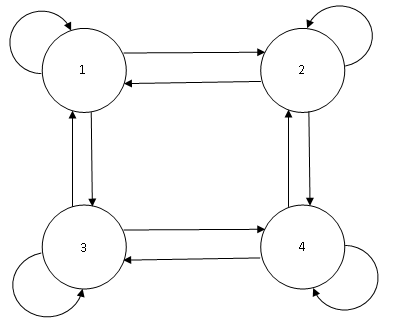
\includegraphics[width=1.0\textwidth]{ThesisFigs/erdogicMC}
                \caption{An Ergodic Markov Chain}
                \label{fig:unclust}
        \end{subfigure} 
        \begin{subfigure}[b]{0.5\textwidth}
                \centering
                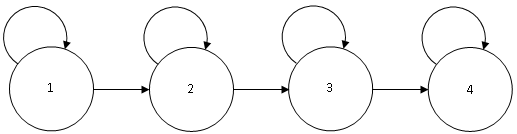
\includegraphics[width=1.0\textwidth]{ThesisFigs/del1LRMC}
                \caption{A $\Delta = 1$ Left-Right Markov Chain}
                \label{fig:clust}
        \end{subfigure}
	   \begin{subfigure}[b]{0.5\textwidth}
                \centering
                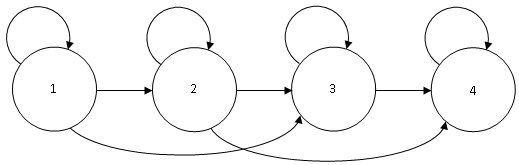
\includegraphics[width=1.0\textwidth]{ThesisFigs/del2LRMC}
                \caption{A $\Delta = 2$ Left-Right Markov Chain}
                \label{fig:clust}
        \end{subfigure}
        \caption{Different Markov Chain Topologies}\label{fig:mctop}
\end{figure}

As such we choose to intialize our HMMs as left-right models restricted to $\Delta = 1$ and initialise the stochastic matrix with form
\begin{equation*}
A =
 \begin{pmatrix}
  a_{11} & a_{12} & 0 & \cdots & 0 \\
  0 & a_{22} & a_{23} &\cdots & 0 \\
  \vdots  & \vdots  & \vdots & \ddots & \vdots  \\
  0 & 0 & \cdots & a_{(n-1)(n-1)}& a_{(n-1)n} \\
  0 & 0 & \cdots & 0& 1
 \end{pmatrix}
\end{equation*}
and define $\pi = [1,0, \dots, 0]$. Clearly if we initialise the non-zero $a_{ij}$ of A deterministically then we restrict ourselves to single outcome from the re-estimation procedure regardless of how many times we retry it, as such we choose to introduce some stochasticity by setting
\begin{align*}
&a_{ii} = 0.5 - r &a_{i(i+1)} = 0.5 + r
\end{align*}
 for some $r$ chosen uniformly from the interval $[-0.3, +0.3]$. This interval is chosen to ensure that none of the links are set too weakly and the forward transitions broken during re-estimation.

As we expect the system to differentiate a large number of signs it would be a major task to taylor the initialistions of each Hidden Markov Model to the sign it is expected to recognise. Hence, we choose to use the same initial estimation procedure for each HMM and do not make any inferences about the structure of the emissions matrix $B$ given the sign it is expected model. We initialise $B$ almost uniformly with
\begin{align*}
&b_{ij} = 1/M + r_{ij} &\text{for each $1\leq i \leq N$ and $1 \leq j \leq M$}
\end{align*}
where each $r_{ij}$ is some small random number and subject to the condition that the matrix $B$ remains stochastic.

The benefit of introducing stochasticity into the initial parameter estimations is that if the re-estimation procedure does not produce a sufficiently good parameterisation we can re-initialise our HMM and try again. That is to say we may use the forward-backward algorithm as part of a random restart hill climbing algorithm~\citep{russell1995artificial} to increase the chances that we will find a good parameterisation for the model.

\section{Observation Vector Quantization}
In order to use discrete observation hidden markov models for the problem of gesture recognition we must restrict the continuous observation space to a discrete set of observation symbols. This set of symbols should not be too large (say no more than 30 symbols) to ensure that the problems of training and evaluation can be solved quickly enough for use in a real-time recognition system. Further, an increase in the number of symbols will cause a decrease in the evaluated probability of a given observation sequence being generated by some HMM. If the symbol count is too high this can cause underflow in spite of the effects of scaling. Of course the symbol set should not be too small either as otherwise we might lose some subtle aspects of signs and cause similar signs to be indistinguishable.

To quantize our training data we merged all of the points of all of the available training data into a single 3D point cloud and partitioned this point cloud into $k$ clusters. To do this we implemented Lloyd's algorithm to solve the k-means clustering problem. Then for any point we can assign an observation symbol in the range $\{1,\dots,k+1\}$ by taking the number of the cluster with the centroid closest (via Euclidean distance) to the point, or if the distance from the point to each of the means exceeds some threshold assigning the symbol $k+1$. 

\begin{figure}[h!]
        \centering
        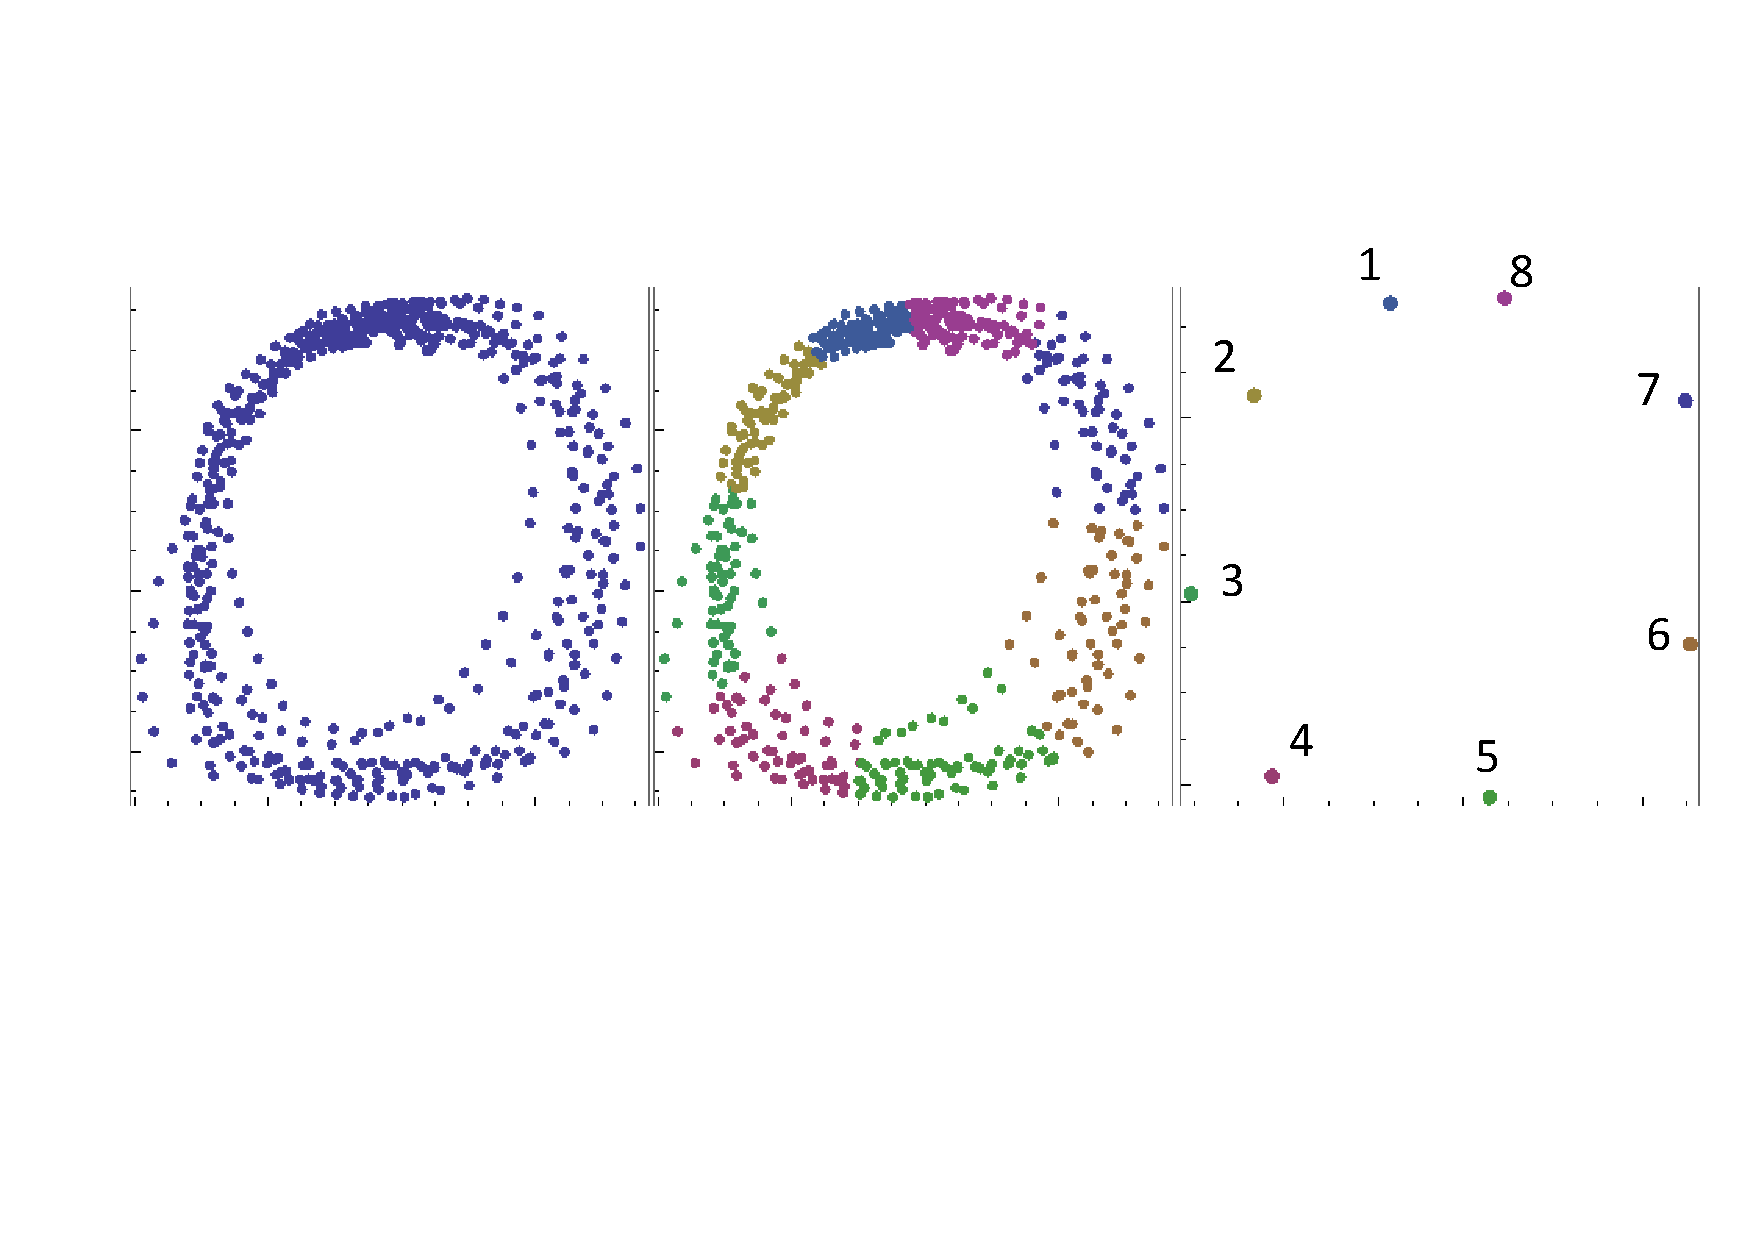
\includegraphics[width=0.9\textwidth]{ThesisFigs/ClusteringDiag}
        \caption{The K-Means method for vector quantization}\label{fig:kmeans}
\end{figure}

\section{Predicting the Probability of a Sign}
Using the work of the previous sections we implemented a class \verb|DHMM| (Figure: ~\ref{fig:dhmmdiag}) which can be instantiated to model a discrete observation Hidden Markov Model by providing initial parameters $A$, $B$ and $\pi$ along with a collection of less than $M$ vectors \verb|centroids| which are used to translate observations from $\mathbb{R}^n$ (for any $n$) into discrete observations in the \verb|convertToSymbol| method. For convenience we provided a means to save and load these parameters from file which means we need only go through the computationally expensive task of training the model once.

\begin{figure}[h!]
        \centering
        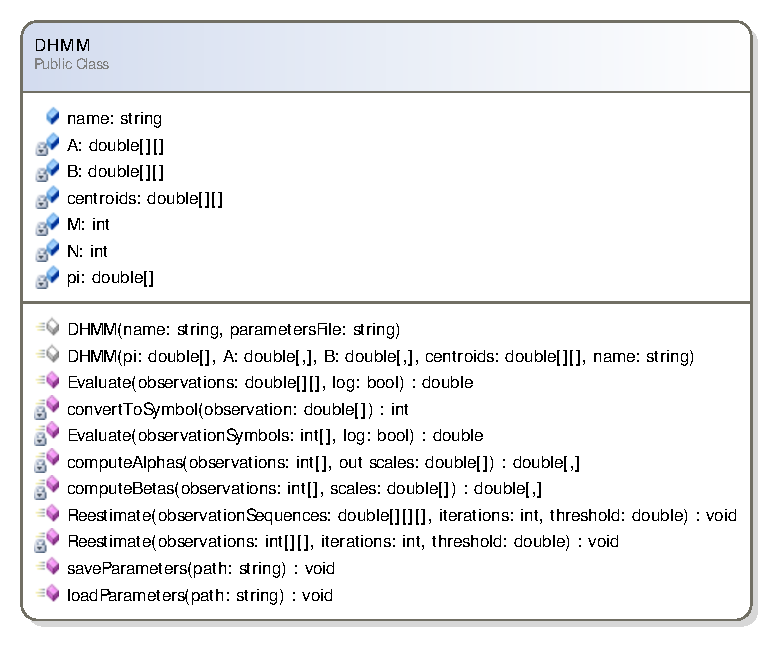
\includegraphics[width=0.9\textwidth]{ThesisFigs/DHMMDiag}
        \caption{A UML skeleton of the DHMM class}\label{fig:dhmmdiag}
\end{figure}

The Kinect Sensor provides a stream of real-time positions, as vectors in $\mathbb{R}^3$, of a number of joints in the body. A single \verb|DHMM| object can be trained on a collection of observations sequences of one of these joints, the left hand say, and be used to determine the probability that another observation sequence was produced by that HMM. If this probability is high enough we might conclude that this observations sequence matches the sign that produced the training data, however this procedure will only use observations from the left hand and ignore the information provided by the rest of the body.

One solution to this problem is to create an instance \verb|DHMM| which takes as its input streams vectors of $(\mathbb{R}^3)^J$ where $J$ is the number of joints we choose to track. This will allow us to train the model on full observations of the body and hence will take into account all of the information available through the Kinect Sensor in computing the probability that an observation sequence corresponds to a specific sign. This method introduces two problems however. The first is purely practical - the computations in the k-means clustering and training algorithms will become more and more expensive as the dimension of the observation vector grows and this will impact negatively on the perfomance of our sign recognition system.

The second issue is that this method ignores the prior knowledge we have about the joints of that body - that some are more dominant in the expression of a sign than others. For example, we know that the right hand is more dominant than the left and that both are more dominant than the elbows or shoulders. In fact the elbows and shoulders might be only worth considering when the hands alone cannot used to determine two different signs. As such we should not let the importance of each joint be determined algorithmically and should specify these parameters with care. For this we create $J$ seperate instances of \verb|DHMM|, each trained on a collection of observations sequences of a different joint. Then supposing we have trained a set of Hidden Markov Models $\Lambda = \{\lambda_1, \dots, \lambda_J\}$ for each joint, and observations sequences $\mathcal{O} = \{\mathbf{O}_1,\dots, \mathbf{O}_J\}$ which specify a stream for each joint over the course of one sign, we can compute the log-probability that this sequence corresponds to the sign used to train $\lambda_1, \dots, \lambda_J$ as a weighted sum
\begin{equation*}
\log(\mathbf{P}[\mathcal{O} | \Lambda ]) = \sum_{j=1}^{J} c_j \log(\mathbf{P}[\mathbf{O}_j | \lambda_j])
\end{equation*}
Where the weights $c_j$ are used to express the dominance of the $j^\text{th}$ joint in expressing a sign relative to the other joints.

We implemented the class \verb|SignModel| (Figure:~\ref{fig:signModel}) to correspond to this definition of $\Lambda$. This class contains a collection of \verb|DHMM| objects with each corresponding to a joint of the skeleton provided by the Kinect Sensor, as well as a set of weightings corresponding to the $c_1, \dots c_J$. This class contains a method \verb|trainClassifier| which will train an instance of \verb|DHMM| for each training data file in /signAlign/Data/Training/name where "name" is the name of the sign. The \verb|trainClassifier| class also contains a method to compute the probability that a given collection of joint observation sequences corresponds to this sign using the weighted sum of joints method described above.
\begin{figure}
        \centering
        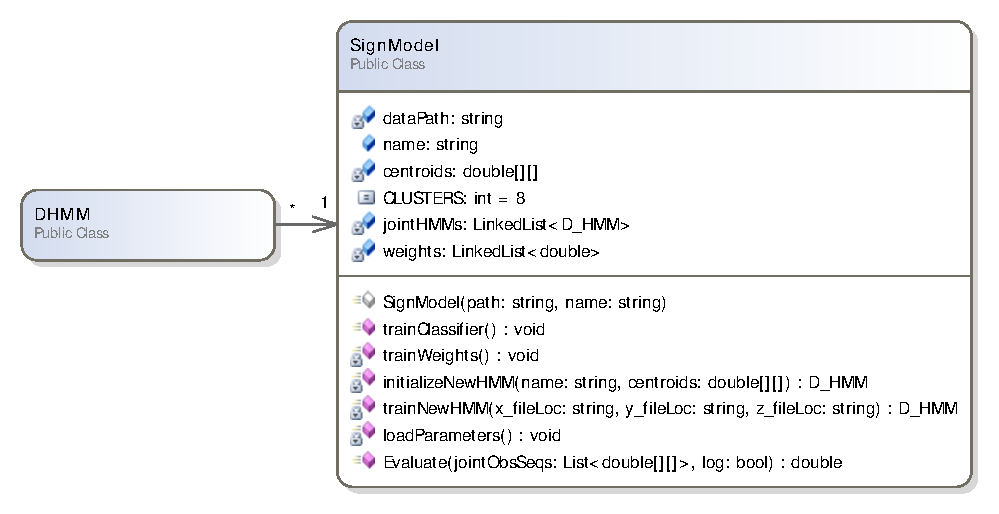
\includegraphics[width=0.9\textwidth]{ThesisFigs/signModelDiag}
        \caption{A UML diagram for the signModel class}\label{fig:signModel}
\end{figure}

\subsection{Determining the Weightings}


\section{Building a Sign Classifier}
A \verb|signModel| object, when trained using suitable of training data from a single sign, allows us to evaluate how likely a new observation sequence is to have been produced by that instance of \verb|signModel| and hence how likely that new observation sequence is to be an instance of the sign used to train the model. Hence if we have a trained \verb|signModel| $m_s$ instance for each sign $s$ in some dictionary $D$ and a collection of joint observation sequences $\mathcal{O} = \{\mathbf{O}_1, \dots, \mathbf{O}_J\}$ read from the Kinect Sensor then we can determine which sign model was most likely to have generated $\mathcal{O}$ as
\begin{equation*}
m = \text{argmax}_{s \in D}\{ \mathbb{P}[\mathcal{O}|m_s]  \}
\end{equation*}
where the value $\mathbb{P}[\mathcal{O}|m_s]$ can be computed as above. Then if $\mathbb{P}[\mathcal{O}|m]$ is sufficiently large then we can conclude that $\mathcal{O}$ corresponds to the sign used to train $m$.
% ------------------------------------------------------------------------

%%% Local Variables: 
%%% mode: latex
%%% TeX-master: "../thesis"
%%% End: 
